\chapter{Éléments théoriques sur la méthode de champ de phase}
\section{Présentation des principales méthodes de suivi et de capture d'interface}

Le traitement numérique efficace des interfaces représente un enjeu majeur de la simulation numérique tant les application faisant intervenir des interfaces sont importantes, de nombreuses méthodes existent mais les principales étant :
\begin{itemize}
	\item[$\bullet$] \textit{\textbf{Volume of fluid (VOF) : }} Cette méthode utilise un maillage fixe découpé en cellule représentant des volumes. On associe alors à chacune de ces cellule une fraction volumique de fluide, cette proportion est alors résolu au cours du temps et la position de l'interface peut être reconstruite. Cette reconstruction a pour désavantage de ne fournir que peu d'informations viables sur l'interface. Cette méthode reste donc peu précise et est également difficile à mettre en \oe uvre en trois dimensions.
	\item[$\bullet$] \textit{\textbf{Méthode Level-Set : }}	Cette méthode repose sur la résolution implicite de l'interface au travers de la résolution d'une fonction auxiliare dite fonction ligne de niveau, généralement la distance signée à l'interface. Cette fonction se doit d'admettre une valeur nulle à l'interface, ainsi au travers de la résolution d'une équation d'advection sur cette fonction ligne de niveau, l'interface est résolue. Cette méthode convient pour les problèmes à fort changement topologique mais présente le désavantage d'être non-conservative.
	\item[$\bullet$]\textit{ \textbf{Arbitrary Lagrangian-Eulerian (ALE) : }} La méthode repose sur une double description lagrangienne (maillage mobile) et eulérienne (maillage fixe), à chaque itération temporelle, le maillage autour de l'interface est reconstruit pour s'adapter à la forme de l'interface, ainsi chaque maille contient uniquement un fluide. L'ensemble de ces propriété rend la méthode très précise mais difficile à mettre en \oe uvre en trois dimensions.
\end{itemize}








\section{Méthode d'interface diffuse}

Les méthodes de suivi d'interfaces peuvent se découper en deux principaux paradigmes concernant le traitement de l'interface, cette dernière peut être raide ou diffuse. Dans le second cas l'interface est modélisée comme une zone de transition d'épaisseur connue entre les deux phases ou les deux fluides cohabitent de manière à ce que les variables observées varient continuellement, facilitant ainsi le traitement numérique de l'interface, les gradients à l'interface n'étant plus infinis. Le concept d'interface diffuse date du XIX-ième siècle et est introduit par Van Der Walls sans susciter d'intérêt jusqu'au années 1950 avec la description de l'énergie libre par Ginzburg et Landau et la description thermodynamique de l'interface en utilisant cette description par Cahn et Hilliard en 1958 et 1959.
\begin{figure}[H]
	\centering
	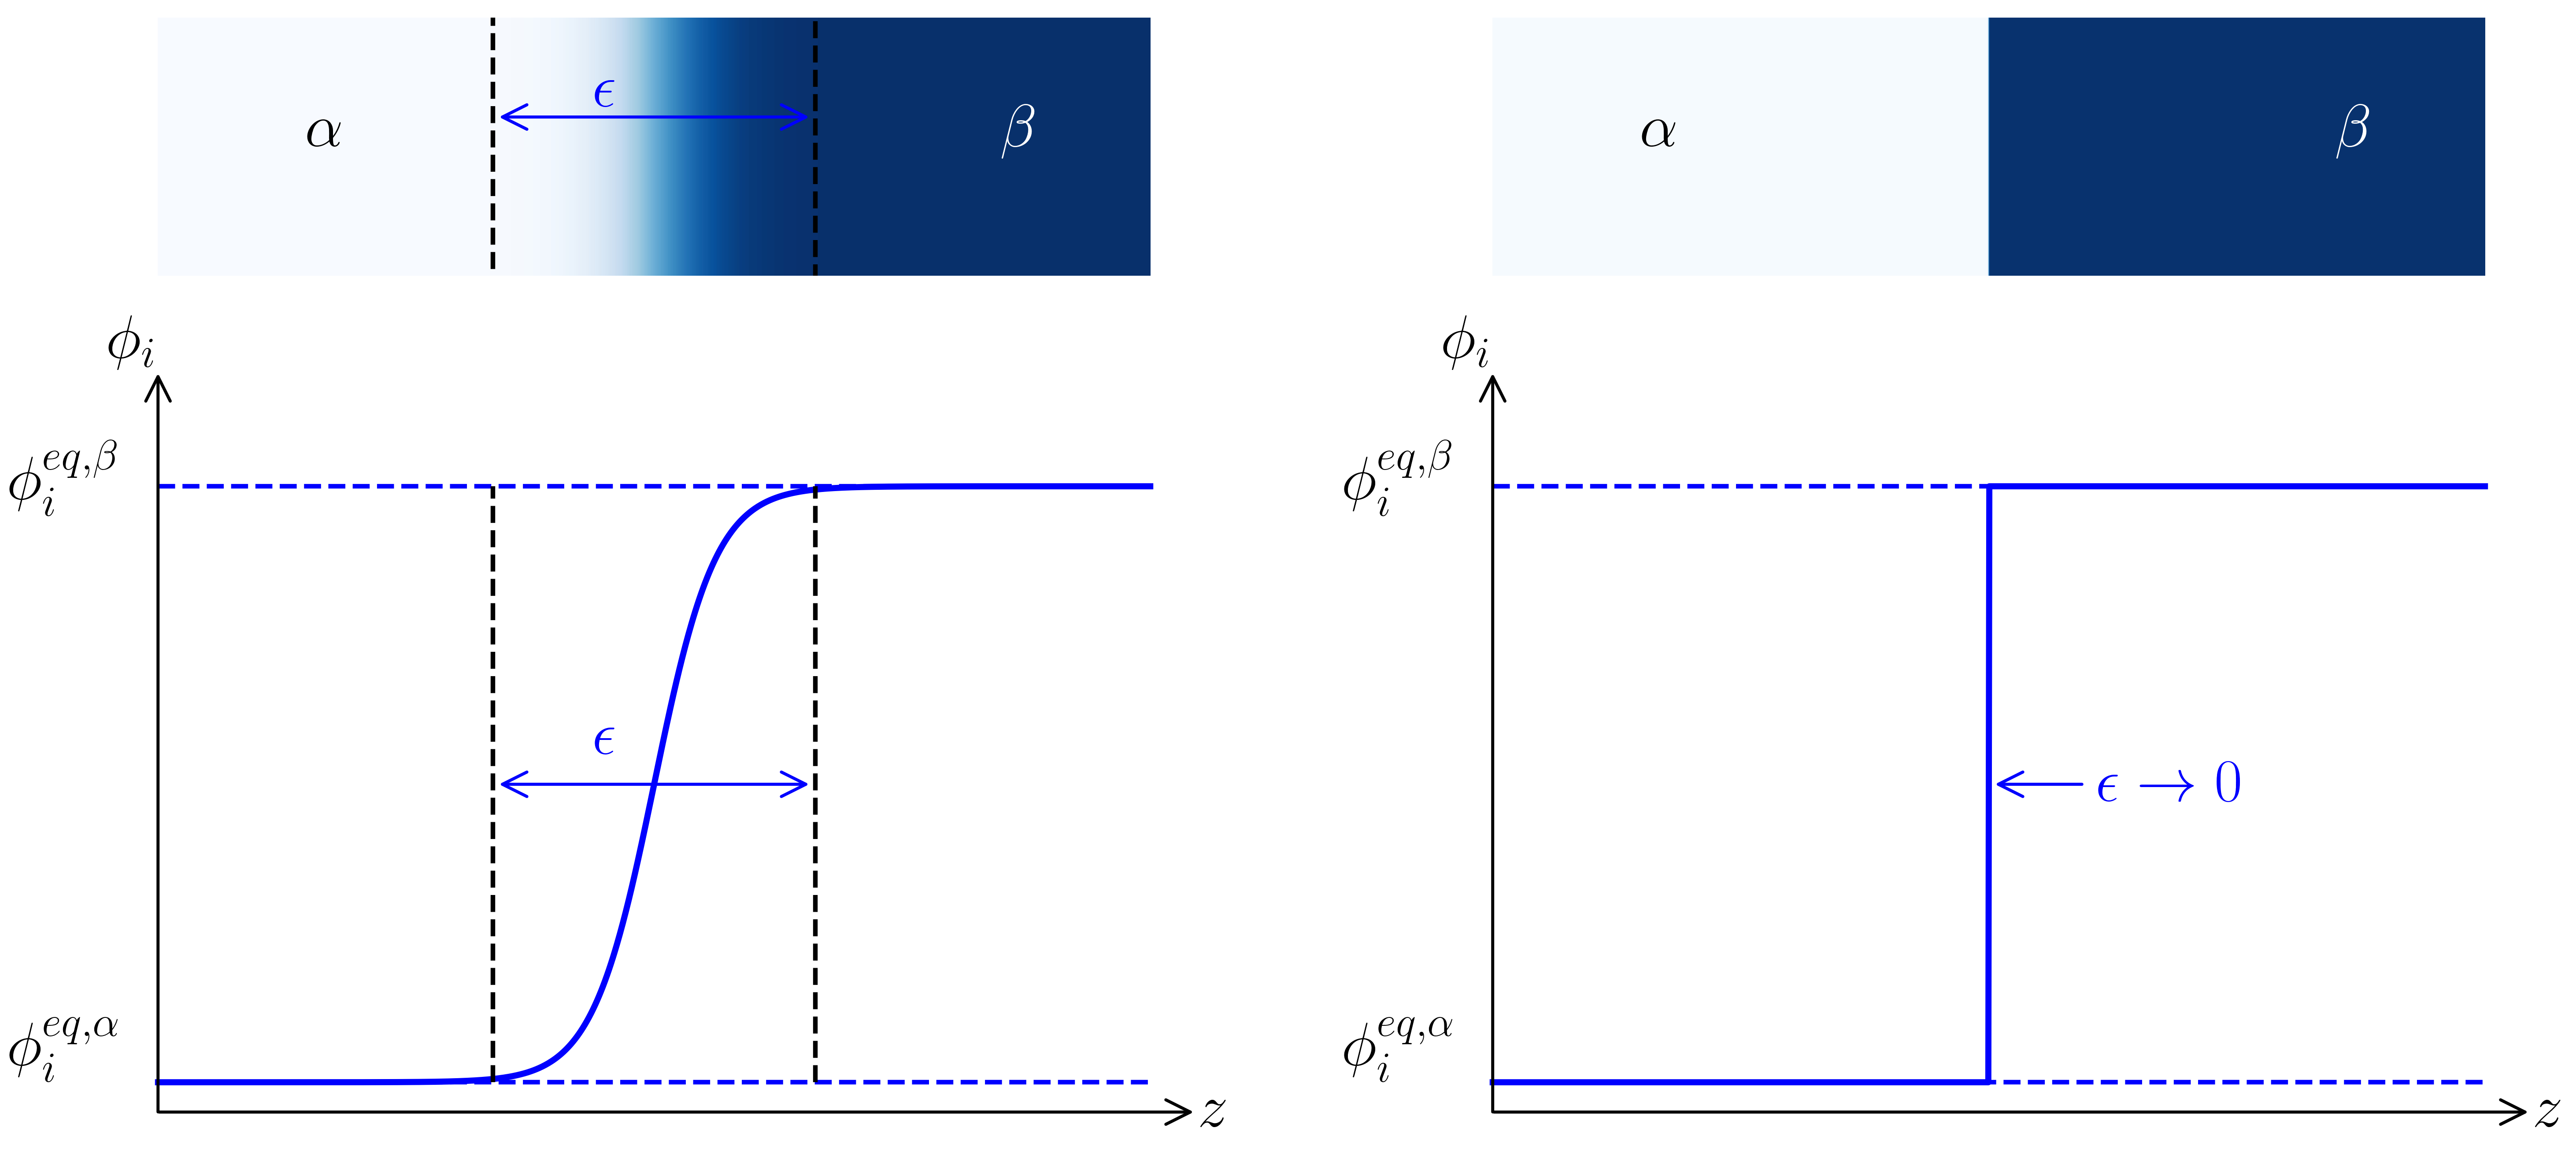
\includegraphics[width=0.7\linewidth]{figure/diffuse_interface}
	\caption{Comparaison entre une interface raide et une interface diffuse}
	\label{fig:diffuseinterface}
\end{figure} 
\noindent L'interface est alors suivie implicitement grâce à une fonction champ de phase qui est définie à partir de grandeurs thermodynamiques. Cette fonction champ de phase prend des valeurs constantes et connues dans chaque phase. Dans la suite on notera cette variable champ de phase $\phi$. Cette méthode est utilisée dans de nombreux domaines.

\begin{figure}[H]
	\centering
	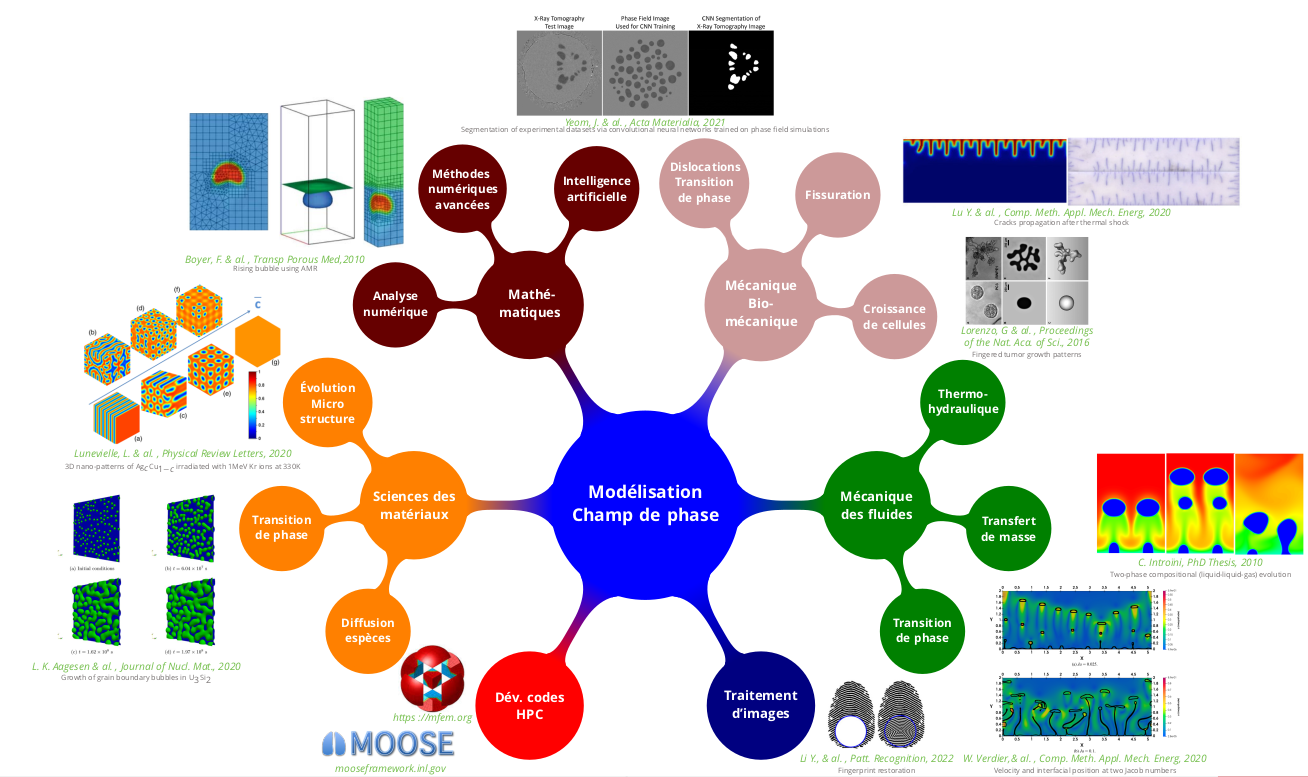
\includegraphics[width=0.9\linewidth]{figure/champ_phase}
	\caption[Domaine d'application de la méthode champ de phase]{Domaine d'application de la méthode champ de phase, tirée de \cite{introini_suivi_nodate}}
	\label{fig:champphase}
\end{figure} 
\section{Équation de Cahn-Hilliard généralisée}
Comme expliqué précédemment la méthode de champ de phase repose sur le suivi d'une variable de phase (ou paramètre d'ordre) noté $\phi_i$ pour la phase $i$ et contraint tel que : 
\begin{equation}
\sum_i \phi_i =1 \Rightarrow \phi_n =1 - \sum_{i=1}^{n-1} \phi_i
\end{equation} 
Ainsi pour un mélange à $n$ composants, seul $n-1$ variables sont indépendantes et autant d'équations de Cahn-Hilliard sont à écrire. Dans certains cas le système peut également être décrit avec des variables non conservées telles que des indicatrices de phases ou des grandeurs liées à des réactions chimiques, les comportements de ces variables sont alors régis par une équation de réaction-diffusion dite d'Allen-Cahn, dans notre étude cette équation ne sera pas résolue car l'ensemble des paramètres d'ordre sont conservés. Dans le cadre de variables conservées les équations de Cahn-Hillard pour $n$ composants, avec $i\in \{1,..,n-1 \}$ s'écrivent sous la forme :
\begin{equation}
\cfrac{\partial \phi_i}{\partial t} + \left(\mathbf{u} \cdot \nabla\right) \phi_i=  \nabla \cdot \left(\sum_{j=1}^{n-1}{\mathcal{M}_{ij}} \nabla\left( \frac{\partial \mathbb{F}}{\partial \phi_j}\right) \right) 
\end{equation}
avec : $\mathcal{M}_{ik}$ la mobilité (paramètre cinétique),  $\phi$ le paramètre d'ordre, $\mathbf{u}$ la vitesse et $\mathbb{F}$ une fonctionnelle de Ginzburg-Landeau généralisée \cite{cardon_modelisation_2016} définit tel que : 
 \begin{equation}
\mathbb{F}[\phi_1,..,\phi_n] = \int_{\mathcal{V}}\tilde{f}_0(\bm{\phi},\mathbf{x},t)+ \sum_{i=1}^{n-1}\sum_{j=1}^{n-1}\cfrac{\kappa_{ij}}{2}\nabla \phi_i \cdot \nabla \phi_j dV
\end{equation}
Où le premier terme représente la densité d'énergie liée aux valeurs locales de composition, traduisant l'équilibre des phases ainsi que leurs existences ou coexistence. Pour deux phases $\alpha$ et $\beta$, on rappel l'équilibre thermodynamique donné par :
\begin{subequations}
	\begin{align}
		&\left.\frac{\partial \tilde{f}}{\partial \phi_i}\right|_{\phi_i^{\alpha,eq}} = \left.\frac{\partial \tilde{f}}{\partial \phi_i}\right|_{\phi_i^{\beta,eq}} = \tilde{\mu}_i^{eq} \hspace{1cm} \Leftrightarrow   \hspace{1cm} \tilde{\mu}_i^{\alpha,eq} = \tilde{\mu}_i^{\beta,eq} \\
		& 		\tilde{f}_0^{\alpha,eq} - \sum_{i=1}^{n-1}\tilde{\mu}_i^{eq}\phi_i^{\alpha,eq} = 	\tilde{f}_0^{\beta,eq} - \sum_{i=1}^{n-1}\tilde{\mu}_i^{eq}\phi_i^{\beta,eq}
	\end{align} 
\end{subequations}
Le second terme représente la contribution des interfaces, le coefficient $\kappa$, dit coefficient de gradient, tient compte du coût énergétique engendré par l'interface, par la suite ce paramètre pourra être relié à la tension de surface. \\
Finalement la dérivé variationnelle de cette fonctionnelle d'énergie libre peut être définit comme un potentiel de diffusion $\tilde{\mu}$: 
\begin{equation}\label{eq_potentiel}
	\frac{\partial \mathbb{F}}{\partial \phi_j} =\lambda \frac{\partial \tilde{f}_0}{\partial \phi_j} -\sum_{k=1}^{n-1} \kappa_{jk} \Delta \phi_k = \tilde{\mu}_j
\end{equation}
avec $\lambda$ un paramètre d'upscalling numérique ajouté pour augmenter l'épaisseur de l'interface, dans le cas où $\lambda=1$ l'interface est d'épaisseur "réelle" soit de l'ordre de l'angstr\oe m, les capacités de calcul ne permettant pas de pouvoir faire des calculs avec des maillages contenant de si petits éléments. \\
Le potentiel de diffusion peut être relier au potentiel chimique tel que :
\begin{equation}
	\tilde{\mu}_i = \frac{1}{V_m}\left(\mu_i - \mu_n\right)
\end{equation}
Avec $\tilde{\mu}_i$ (en J.m$^{-3}$) représente le potentiel de diffusion de l'élément $i$, et $V_m$ le volume molaire supposé constant dans tout le système.\\
Le potentiel chimique étant classiquement définit tel que :
\begin{equation}
	\mu_i = \left.\frac{\partial G}{\partial n_i}\right|_{P,T,n_{j\neq i }} = \left.\frac{\partial F}{\partial n_i}\right|_{V,T,n_{j\neq i }}
	  \textrm{                        où           } F = V_m f_0
\end{equation}
Avec $F$ (resp. $G$) l'énergie libre d'Helmotz (resp. Gibbs) (en J) et $n_i$ la quantité de matière de l'élément $i$ (en mol). Dans notre cas on se place dans une transformation isobare et isotherme, on privilégiera donc l'énergie de libre de Gibbs.
Dans le cas où $\doubleoverline{\kappa}$ = $\doubleoverline{0}$ on retrouve une équation d'advection-diffusion classique, dans le cas contraire on obtient une équation d'ordre 4. Une des principale difficulté dans la mise en place de méthode champ de phase repose sur le paramétrage des simulations.
\section{Couplage avec les équations de Navier-Stokes incompressible}
Dans le cadre de cette étude les équations de Cahn-Hilliard sont couplées aux équations de conservation de masse et de quantité de mouvement incompressible sous l'approximation de Boussinesq, d'après \cite{kim_phase-field_2012} le système d'équations s'écrit sous la forme :
\begin{subequations}
\begin{align}
&\nabla \cdot \mathbf{u} = 0\\
&\rho^* \left (\frac{\partial \mathbf{u}}{\partial t} + (\mathbf{u} \cdot {\nabla})\mathbf{u}\right) = -{\nabla} P +\eta \Delta \mathbf{u}+\sum_{i=1}^{n-1} \tilde{\mu}_i{\nabla} \phi_i + \rho(\bm{\phi}) \mathbf{g}
\end{align}
\end{subequations}
avec $\mathbf{u}$ la vitesse, $P$ la pression, $\mu_i$ le potentiel chimique du composant $i$, $\mathbf{g} = \{ 0,0,-g\}^T $, $\eta$ la viscosité cinématique supposée constante, $\rho^*$ la masse volumique du solvant \\
La densité est alors calculé : 
\begin{equation}
	\rho(\bm{\phi}) = \rho^*\left(1+\sum_{i=1}^{n-1}\beta_i \phi_i\right)
\end{equation}
Les paramètres $\beta$ sont à déterminer en fonction du système étudié, $\rho_0$ correspond à une masse volumique de référence. L'équation de Cahn-Hilliard étant d'ordre 4, une résolution implicite est alors préférée pour les simulations.
\section{Paysage thermodynamique analytique}
L'objectif présenté dans \cite{noauthor_numerical_nodate} est de d'obtenir une formulation analytique du terme homogène de la fonctionnelle de Ginzburg-Landau. Dans le cas binaire, cette contribution est de la forme d'un double puit d'ordre 4.
\begin{figure}[h!]
	\centering
	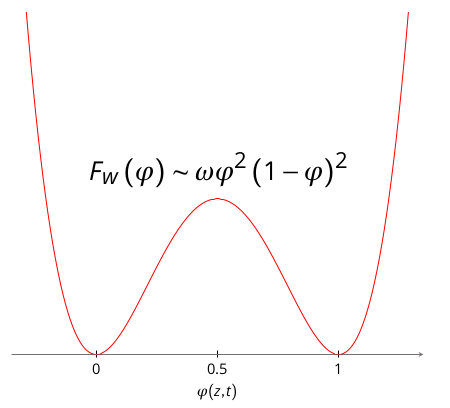
\includegraphics[width=0.4\linewidth]{figure/DP}
	\caption[Exemple d'une contribution homogène à l'énergie]{Exemple d'une contribution homogène à l'énergie, d'après \cite{introini_suivi_nodate}}
	\label{fig:dp}
\end{figure}\\
L'objectif est de généraliser ce double puit pour un système ternaire, ainsi on introduit un pseudo grand potentiel correspondant à l'énergie nécessaire pour changer de minimum d'énergie \cite{cardon_modelisation_2016}.
\begin{equation}
\Omega^{\star} =\Omega - \Omega^{eq} =  \tilde{g}^{liq} - \sum_i \tilde{\mu}_i^{eq}\phi_i - \left(  \tilde{g}^{liq,eq} -  \sum_i \tilde{\mu}_i^{eq}\phi_i^{eq} \right) 
\end{equation}
Les bases thermodynamiques étant peu développées aux points d'intérêt (Température supérieure à 2000 \textdegree C) on cherche à définir ce potentiel grâce à une formulation analytique que l'on note :
\begin{equation}\label{double_puit}
	\Omega^{\star}  = P^{dis} \times P^{cont}
\end{equation}
Où $P^{dis}, P^{cont}$ représente deux paraboloïdes correspondant à la phase dispersée et continue. Dans le cas ternaire, avec les éléments $A$ et $B$ d'intérêt, les paraboloïdes sont de la forme : 
\begin{multline}
	P^{k}=\left(\frac{\co{\theta^{k}}(\phi_{A}-\phi_{A}^{eq,k}) + \sinus{\theta^{k}}(\phi_{B}-\phi_{B}^{eq,k})}{a_{A}^{k}}\right)^{2}+\\ \left(\frac{-\sinus{\theta^{k}}(\phi_{A}-\phi_{A}^{eq,k}) + \co{\theta^{k}}(\phi_{B}-\phi_{B}^{eq,k})}{a_{B}^{k}}\right)^{2}
	\label{eq:paraboloid_general_}
\end{multline} 
Avec $k = \{disp,cont\}$ la phase (dispersée ou continue), $a_A$ (respectivement $a_B$) le demi-grand (resp petit) puits, $\theta_k$ l'angle de rotation associé au puits de la phase $k$\\
On cherche alors à tracer ce paysage.
\begin{figure}[h!]
	\centering
	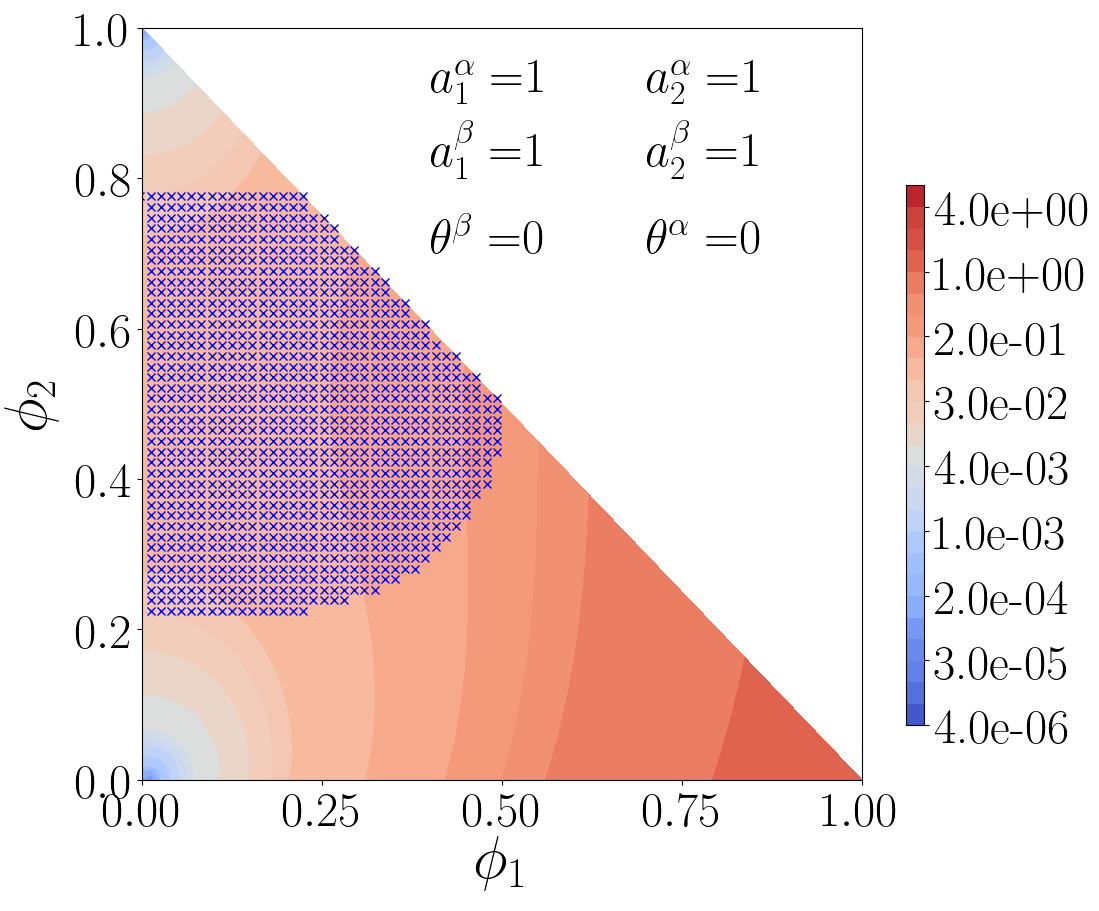
\includegraphics[width=0.7\linewidth]{figure/landscape}
	\caption{Exemple de paysage thermodynamique, en rouge la droite reliant les concentration initiales et en bleu la droite reliant les concentrations à l'équilibre, les pointillés réprésentant la zone instable présenté ci-dessous}
	\label{fig:landscape}
\end{figure}
On peut dès lors calculer le potentiel de diffusion homogène grâce à la formulation analytique (\ref{double_puit}) :
\begin{align}
	\tilde{\mu}_i & \nonumber= \frac{\partial}{\partial \phi_i}\left\lbrace 
	\Omega^{\star} + \sum_j \tilde{\mu}_j^{eq}\phi_j + \left( {g}^{liq,eq} -  \sum_j \tilde{\mu}_j^{eq}\phi_j^{eq} \right)\right\rbrace \\
	&\nonumber = \frac{\partial \Omega^{\star}}{\partial \phi_i} + \frac{\partial g^{liq,eq}}{\partial \phi_i} + \sum_j \frac{\partial \tilde{\mu}_j^{eq}\left(\phi_j - \phi_j^{eq}\right)}{\partial  \phi_i}\\
	\tilde{\mu}_i &=	P^{dis}\frac{\partial P^{cont}}{\partial \phi_i} + P^{cont}\frac{\partial P^{dis}}{\partial \phi_i} + \tilde{\mu}_i^{eq}
\end{align} 
%\begin{align*}
	%& \frac{\partial g^{liq,eq}}{\partial \phi_i} = 0 \\
		%& \sum_j \frac{\partial \tilde{\mu}_j^{eq}\left(\phi_j - %\phi_j^{eq}\right)}{\partial  \phi_i} = \tilde{\mu}_i^{eq} %+\tilde{\mu}_{j\neq i}^{eq} \frac{\partial \phi_{j\neq i}}{\partial %\phi_i} = \tilde{\mu}_i^{eq}
%\end{align*}
L'objectif est alors de déterminer les paramètres des paraboloïdes pour obtenir des résultats consistants thermodynamiquement.
\section{Éléments de stabilité de phase}
Dans le cadre de notre étude nous nous intéressons à deux phases en coexistence, une phase dite continue et l'autre dispersée. La détermination de la stabilité des phases est essentielle pour pouvoir tracer le paysage thermodynamique. La courbe binodale correspond à la condition pour laquelle deux phases peuvent coexister, c'est-à-dire que sous la courbe binodale le système peut être composé d'une seul phase, il le sera dans la zone instable et pourra l'être dans la zone métastable.
\begin{figure}[h!]
	\centering
	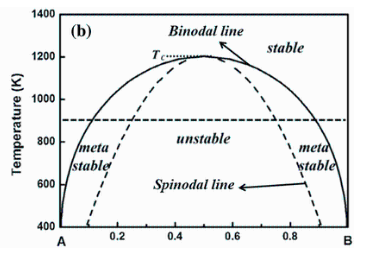
\includegraphics[width=0.5\linewidth]{figure/metastable}
	\caption[Exemple de diagramme de stabilité de phase pour un cas binaire, d'apres]{Exemple de diagramme de stabilité de phase pour un cas binaire, d'apres}
	\label{fig:metastable}
\end{figure}
Cependant le calcul de la zone instable est beaucoup plus simple que celui de la zone métastable. Pour déterminer cette zone instable on calcul la matrice Hessienne définit tel que : 
\begin{equation}
	\Mb{\doubleoverline{H}}_{g^{liq}} = \left.\frac{\partial^2 g^{liq}}{\partial \phi_i \partial \phi_j}\right|_{T,P,\phi_k\neq i,j}
	=\left.\frac{\partial^2 \Omega^{\star}}{\partial \phi_i \partial \phi_j}\right|_{T,P,\phi_k\neq i,j}
\end{equation}
L'égalité des matrices hessienne du pseudo-grand potentiel et de l'énergie libre de Gibbs est ici immédiate. D'après \cite{aursand_spinodal_2017} les zones spinodale, instable et stable sont définit tel que :
\begin{itemize}
	\item zone stable : $\displaystyle eig\left\{\Mb{\doubleoverline{H}}_{g^{liq}} \right\} > 0$, deux phases coexistent \\ 
	\item spinodale : $\displaystyle \min \left( eig \left\{\Mb{\doubleoverline{H}}_{g^{liq}}\right\} \right) > 0$, décomposition spinodale \\
	\item zone instable : $\displaystyle eig\left\{\Mb{\doubleoverline{H}}_{g^{liq}} \right\} < 0$, une phase en présence \\ 
\end{itemize}
Le calcul des valeurs propres en chaque point du paysage pouvant être coûteux on rappel que par théorème le produit des valeurs propres d'une matrice est égale au déterminant de cette matrice. Ainsi si on note $\lambda_i$ les valeurs propres de $\Mb{\doubleoverline{H}}_{g^{liq}}$ on a :
\begin{equation}
	\det{\Mb{\doubleoverline{H}}_{g^{liq}}} = \prod_i \lambda_i
\end{equation}
Pour le cas ternaire le calcul du déterminant est direct :
\begin{equation}
	\text{det}  \Mb{\doubleoverline{H}}_{g^{liq}}   =  \frac{\partial^2 g^{liq}}{\partial \phi_i^2}
	\frac{\partial^2 g^{liq}}{\partial \phi_j^2}-\left(\frac{\partial^2 g^{liq} }{\partial \phi_i \partial \phi_j} \right)^2
\end{equation}
Ainsi la zone instable correspond à la zone où le determinant de la matrice hessienne est négatif.


\section{Expérience numérique}

L'objectif est de réaliser numériquement l'expérience proposée par Abhijit Rao et al. dans \cite{rao_influence_2015}. Pour cette expérience une goutte composée d'Acetonitrile et de Chlorobenzene est placée dans de l'eau. l'acetonitrile est miscible dans l'eau contrairement au chlorobenzene qui est immiscible. Initialement la goutte est plus légère que l'eau environnante et monte puis sous l'effet du transfert de masse la densité de la goutte augmente jusqu’à une inversion du rapport de densité conduisant à la redescente de la goutte.
\subsection{Choix des conditions initiales}
Les conditions initiales choisies pour la concentration sont de la forme tangente hyperbolique.
\begin{equation}
	\phi_{i}(\mathbf{x},t=0) = \frac{\phi^{init,cont}_i + \phi^{init,disp}_i  }{2} +  \frac{\phi^{init,cont}_i - \phi^{init,disp}_i }{2}\tanh\left(\cfrac{\sqrt{(x-x_0)^2+(y-y_0)^2}-R}{\varepsilon} \right)
\end{equation}
Avec ($x_0$, $y_0$) les coordonnées du centre de la goutte, $R$ le rayon de la goutte, $\varepsilon$ l'épaisseur de l'interface (paramètre numérique) et $\phi_i^{init,cont}$ (resp. $\phi_i^{init,disp}$) la concentration initiale de l'élément $i$ dans la phase continue (resp. dispersée) .\\
Cette solution analytique provient d'un problème avec une interface plane (sans courbure), dans la littérature il n'existe pas de solution analytique pour une interface courbée, l'effet de Gibbs-Thomsom n'est donc pas pris en compte, ainsi on observe un léger mouvement de l'interface lors du premier pas de temps. \\
Pour s'assurer de la sphéricité de la goutte lors de la simulation on calcule le nombre adimensionné de Bond  représentant le ratio entre les forces de gravité et la tension de surface tel que :
\begin{equation}
	Bo = \cfrac{\Delta \rho g D^2}{\sigma}
\end{equation}
avec $\Delta\rho$ la différence de densité entre les deux phases, $D$ le diamètre de la goutte et $\sigma$ la tension de surface.\\
On considère que pour $Bo \ll 1$ la tension de surface domine et la goutte reste sphérique.
\begin{figure}[H]
	\centering
	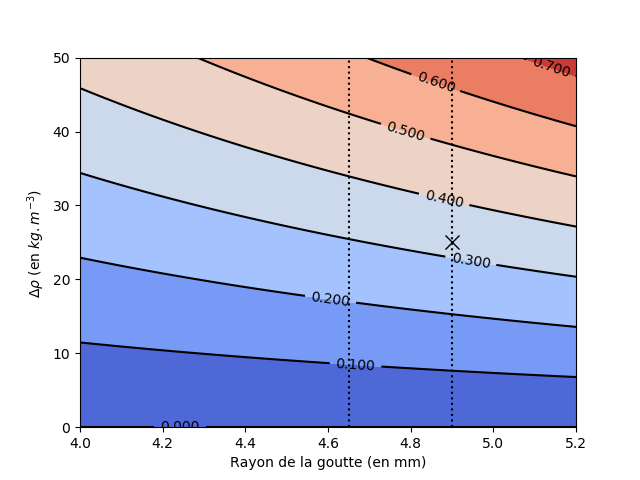
\includegraphics[width=0.7\linewidth]{figure/contour_bond}
	\caption[Valeur du nombre de Bond en fonction de la différence de densité et de la tension de surface entre les phases]{Valeur du nombre de Bond en fonction de la différence de densité entre les phases et le rayon de la goutte, le marqueur représente l'état initial}
	\label{fig:contourbond}
\end{figure}
Il est alors possible, dans notre cas, de discuter de la sphéricité de la goutte au vu de la valeur ici $Bo = 0.32$
